\documentclass{article}
\usepackage{graphicx} % Required for inserting images
\usepackage{titlesec}
\usepackage{tabularx}
\usepackage{makecell} 
\usepackage{array} 
\usepackage{enumitem}
\usepackage{changepage}  
\usepackage{geometry}
\usepackage{float}
\usepackage[none]{hyphenat}
\setcounter{secnumdepth}{4}

\titleformat{\paragraph}
{\normalfont\normalsize\bfseries}{\theparagraph}{1em}{}
\titlespacing*{\paragraph}
{0pt}{3.25ex plus 1ex minus .2ex}{1.5ex plus .2ex}

\title{\textbf{Design Document}}
\author{Armando Fiorini, Samuele Motta, Vajihe Gholami}
\date{}

\begin{document}

\maketitle
\section*{INFO}
\textbf{Deliverable}: DD\\
\textbf{Title}: Design Document\\
\textbf{Authors:} Armando Fiorini, Samuele Motta, Vajihe Gholami\\
\textbf{Version:} 0.0.0\\
\textbf{Date}: 17/12/2023\\
\textbf{Download page}: https://github.com/ArmaFio/FioriniMottaGholami\\
\newpage
\tableofcontents
\newpage

\section{Introduction}
\subsection{Purpose}
The main purpose of the present document is to support the development team in realizing the system. It provides an overall description of the adopted system architecture and a breakdown of the various components to a significant extent, also describing their interactions with each other. On top of that, the Design Document (DD) describes the implementation, integration, and testing plans which are defined keeping into account priority, required effort, and impact of the single components on the stakeholders.

\subsection{Scope}
CodeKataBattle (CKB) helps students improve their software skills through teamwork on coding challenges. It's all about learning together in a fun, competitive way. Educators create tournaments with coding exercises, and students form teams to solve them. The platform handles everything: deadlines, tests, and checking code quality.

Educators can also give personal feedback and scores. CKB is where educators set challenges, students solve them as teams, and everyone can see how they're doing. It handles tournaments, battles, team setups, code submissions via GitHub, live scoring, and awarding badges for achievements.

The system focuses on teamwork, good coding methods using tests, and a mix of competition and support. Automated tools ensure fair assessments while letting educators give helpful feedback. Badges and student profiles make it fun, encouraging everyone to participate and shine. Overall, CKB is a platform mixing learning, teamwork, competition, and skill-building in software development.

\subsection{Definitions, Acronyms, Abbreviations}
\subsubsection{Definitions}
Educator: A user who signs up to use the system to improve his students' programming skills can create Tournaments and badges. \\
Student: user who signs up to improve their skills, and participate in tournaments are created by the educators.\\
Tournament: coding challenge, consisting of a certain number of battles. Team: group of students, formed to join a tournament and work together to win the battles. \\
Battle: every single challenge the tournament is composed of. \\
(Gamification) Badge: achievement that is created by an educator, and can be obtained from Students satisfying the established requirements.\\

\subsubsection{Acronyms}
\begin{itemize}
    \item \textbf{CKB}: CodeKataBattle
    \item \textbf{RASD}: Requirement Analysis and Specification Document
    \item \textbf{UI}: User Interface
    \item \textbf{UML}: Unified Modelling Language
    \item \textbf{OS}: Operative System
\end{itemize}

\subsection{Revision History}
\begin{itemize}
    \item \textbf{$[Gn]$}: the n-th goal of the system.
    \item \textbf{$[Wn]$}: the n-th world phenomena.
    \item \textbf{$[SWn]$}: the n-th shared phenomena controlled by the world.
    \item \textbf{$[SMn]$}: the n-th shared phenomena controlled by the machine.
    \item \textbf{$[Dn]$}: the n-th domain assumption.
    \item \textbf{$[FRn]$}: the n-th functional requirement.
\end{itemize}


\subsection{Reference Documents}
This document is based on:
\begin{itemize}
    \item The specification of the RASD and DD assignment of the Software Engineering II course, held by Professor Matteo Rossi, Elisabetta Di Nitto, and Matteo Camilli at the Politecnico di Milano, A.Y 2023/2024; 
    \item Slides of Software Engineering 2 course on WeBeep;
\end{itemize}


\subsection{Document Structure}
Mainly the current document is divided into 4 chapters, which are:
\begin{itemize}
    \item \textbf{Introduction:} The first chapter includes the introduction which explains the purpose of the document, then, a brief recall of the concepts introduced in the RASD is given. Finally, important information for the reader is given, i.e. definitions, acronyms, synonyms, and the set of documents referenced. 
    \item \textbf{Architectural Design:} It includes a detailed description of the architecture of the system, including the high-level view of the elements, the software components of …, a description through run-time diagrams of various functionalities of the system, and, finally, an in-depth explanation of the architectural pattern used.
    \item \textbf{User Interface Design:} Provide mockups of the application user interfaces, with the links between them to help in understanding the flow between them. 
    \item \textbf{Requirements Traceability:} It describes the connections between the requirements defined in the RASD and the components described in the first chapter. This is used as proof that the design decisions have been taken concerning the requirements, and therefore that the designed system can fulfill the goals. 
    \item \textbf{Implementation, Integration, and Test Plan:} It describes the process of implementation, integration, and testing to which developers have to stick to produce the correct system correctly. 
    \item \textbf{Effort Spent:} Contains information about the time spent to create this document. 
    \item \textbf{References:} It contains the references to any documents and the Software used in this document. 
\end{itemize}
\section{Architectural Design}

\subsection{Overview}
This section gives an overview of the architectural elements that compose the system, their interaction, and a description of the replication mechanism chosen for the system to make it distributed.
\subsection{High-Level view}

The CodeKataBattle project follows a 3-tier architecture, segregating its functionalities into distinct layers. (Figure \ref{fig:3-tier}) The Presentation Layer handles the user interface, authentication, notifications, and badge visualization. The Application Layer contains the core logic, managing battles, tournaments, GitHub integration, score calculation, and badge generation. The Data Layer ensures data integrity and storage, interacting with the database and employing ORM for data operations. Communication between these tiers occurs through APIs or service calls. This modular structure streamlines development, fostering scalability and maintainability. The front end allows user interaction while the back end manages logic, data, and integrations, providing educators and students with a seamless platform to engage in code kata battles and tournaments, track progress, and visualize achievements through earned badges.

\begin{figure}[H]
    \centering
    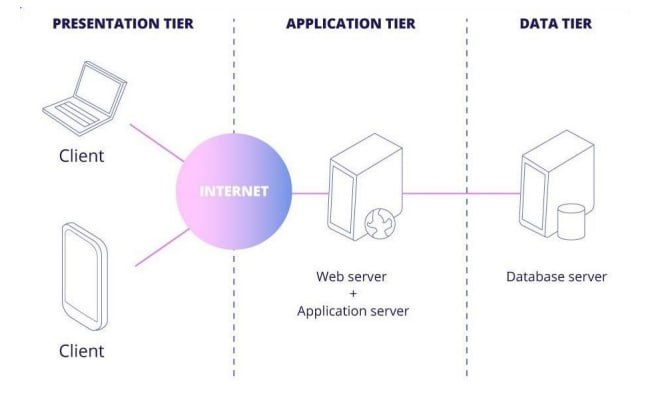
\includegraphics[width=\linewidth]{High level view.jpg}
    \caption{3-tier architecture}
    \label{fig:3-tier}
\end{figure}

Regardless of whether the user is an educator or a student, they can access the application through either the web or mobile app, with communication between the client and server relying on various components tailored to the consumer device's type.

\subsection{Distributed View}
\subsection{Component view}

\begin{figure}[H]
    \centering
    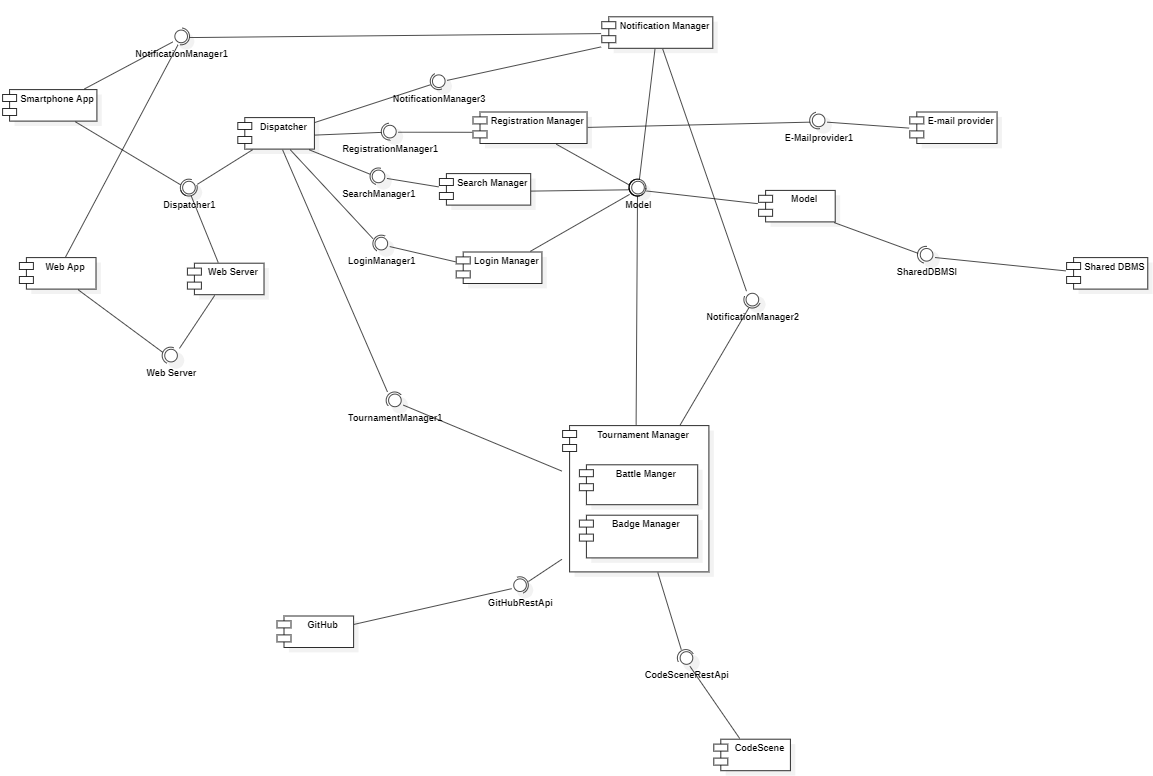
\includegraphics[width=\linewidth]{Component diagram.png}
    \caption{Component Diagram}
\end{figure}

\subsection{Deployment view}

\subsection{Runtime view}
It's crucial to clarify a key point about the following sequence diagrams: the system can be accessed through both a mobile app and a web app. For simplicity, we've unified the representation of the web app and mobile app under the \textbf{App} component, omitting the web server. It's implicit that when using the web app, all requests pass through the web server before reaching other components.

\begin{figure}[H]
    \centering
    \textbf{[UC11] Manual Evaluation} \\
    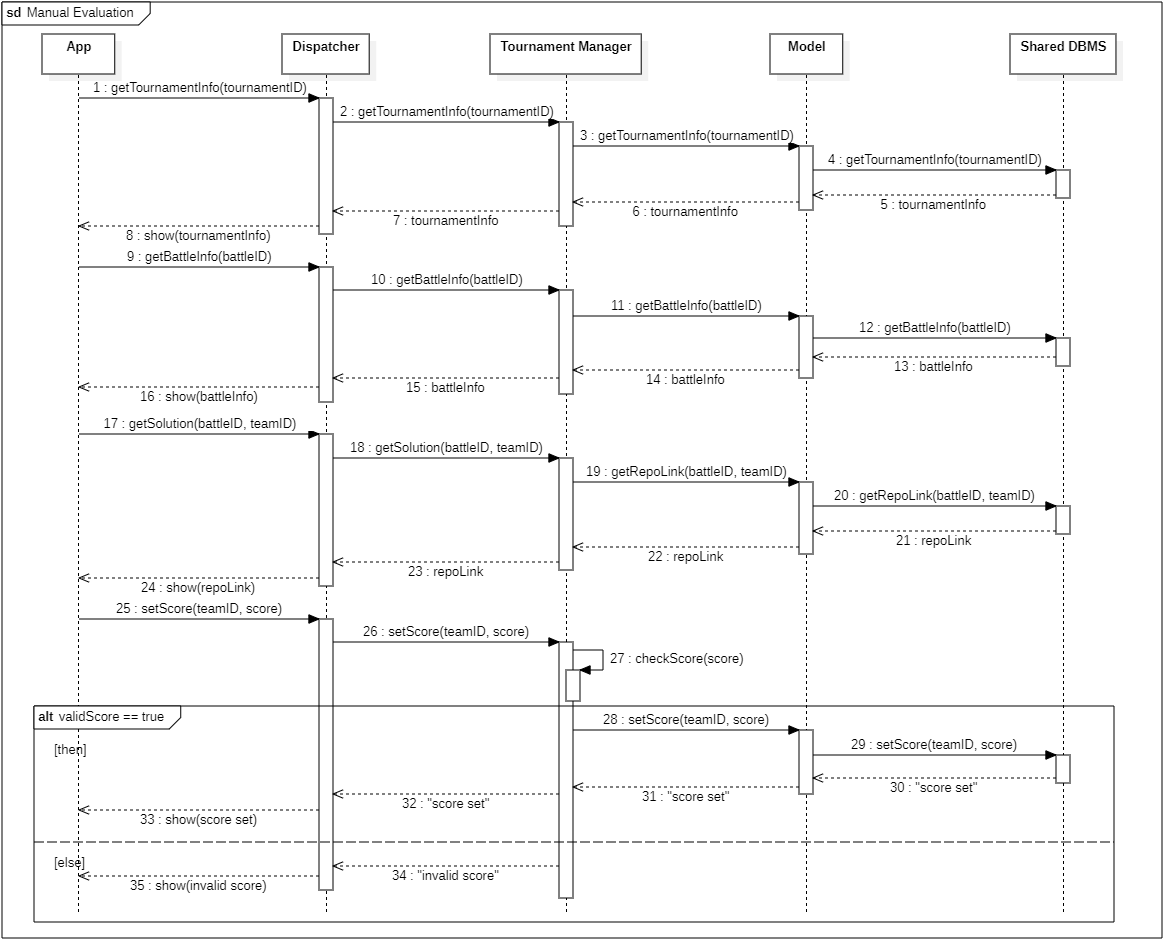
\includegraphics[width=\linewidth]{UC11.png}
\end{figure}
\noindent
This sequence diagram depicts the manual evaluation process conducted by an educator. The app initiates the procedure by sending the dispatcher a request to obtain information about a specific tournament. This request is then forwarded to the Tournament Manager, and subsequently to the Model and the Shared DBMS. \\
Once the tournament information has been retrieved, a new request is sent to the Shared DBMS to retrieve information about a specific battle within the tournament. Following this, another request is made to obtain the solution of a specific team within the battle. \\
The educator assesses the solution and assigns a score, which the Tournament Manager then verifies. If the score is deemed valid, the Tournament Manager proceeds to set the score for the solution in the Shared DBMS. Otherwise, it returns an error message to the app. \\


\begin{figure}[H]
    \centering
    \textbf{[UC12] Fork Creation} \\
    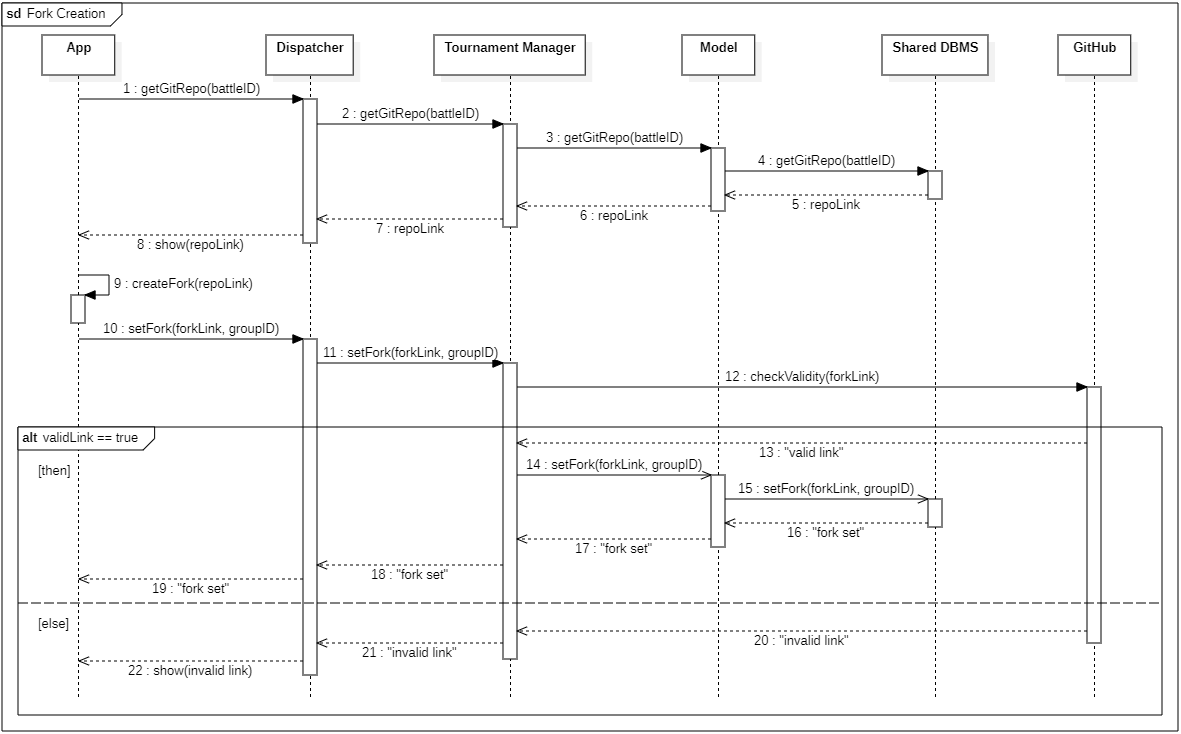
\includegraphics[width=\linewidth]{UC12.png}
\end{figure}
\noindent
This sequence diagram illustrates the fork creation process carried out by a student. The procedure commences with the app sending a request to obtain the repository link containing the problem for a specific battle. The Tournament Manager then retrieves this link from the Shared DBMS. \\
Subsequently, the student creates a new fork by accessing the GitHub repository through the provided link. The student then submits the link of the new fork to the system for processing. The Tournament Manager, in turn, interacts with the GitHub API to validate the link provided by the student. If the link is valid, the Tournament Manager saves it in the Shared DBMS and sends a confirmation message to the user. However, if the link is invalid, the system sends an error message to the user.

\begin{figure}[H]
    \centering
    \textbf{[UC13] Close Tournament} \\
    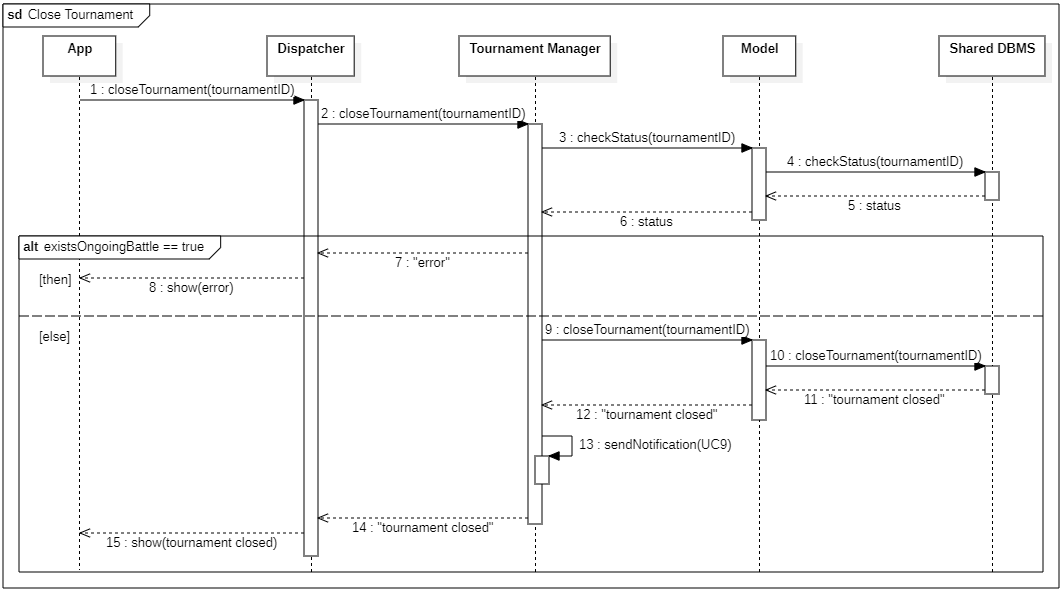
\includegraphics[width=\linewidth]{UC13.png}
\end{figure}
\noindent
This sequence diagram represents the procedure for closing a tournament, executed by the educator who created it. Initially, the app sends a request to close the tournament to the Tournament Manager, which then verifies the tournament's state through the Shared DBMS. If there are no ongoing battles within the tournament, the Tournament Manager updates the tournament state to 'closed' in the Shared DBMS and notifies all students who joined that tournament via the Notification Manager. However, if there are ongoing battles, an error message is sent to the app.

\begin{figure}[H]
    \centering
    \textbf{[UC14] Visit Profile} \\
    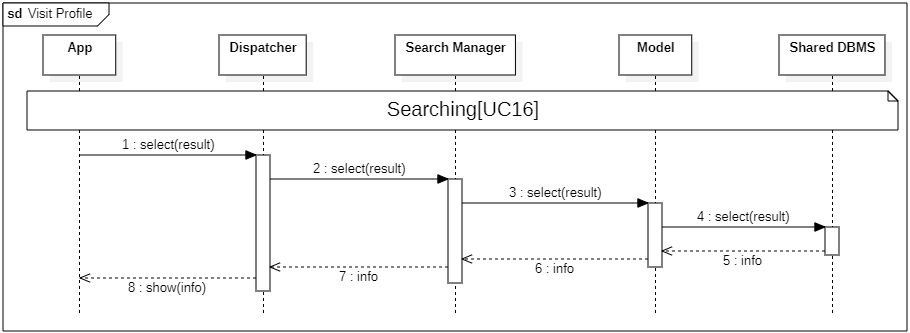
\includegraphics[width=\linewidth]{UC14.png}
\end{figure}
\noindent
This sequence diagram illustrates the process of visiting a user profile. It begins with the app initiating a request to retrieve information about a specific keyword, as described in \textbf{[UC16]}. Following the retrieval of suggested results, the app sends the selected topic to the Search Manager for information retrieval. The Search Manager then collects the information by querying the Shared DBMS. Finally, all the gathered information is sent back to the Search Manager and subsequently to the app.

\begin{figure}[H]
    \centering
    \textbf{[UC15] Joining Invitation} \\
    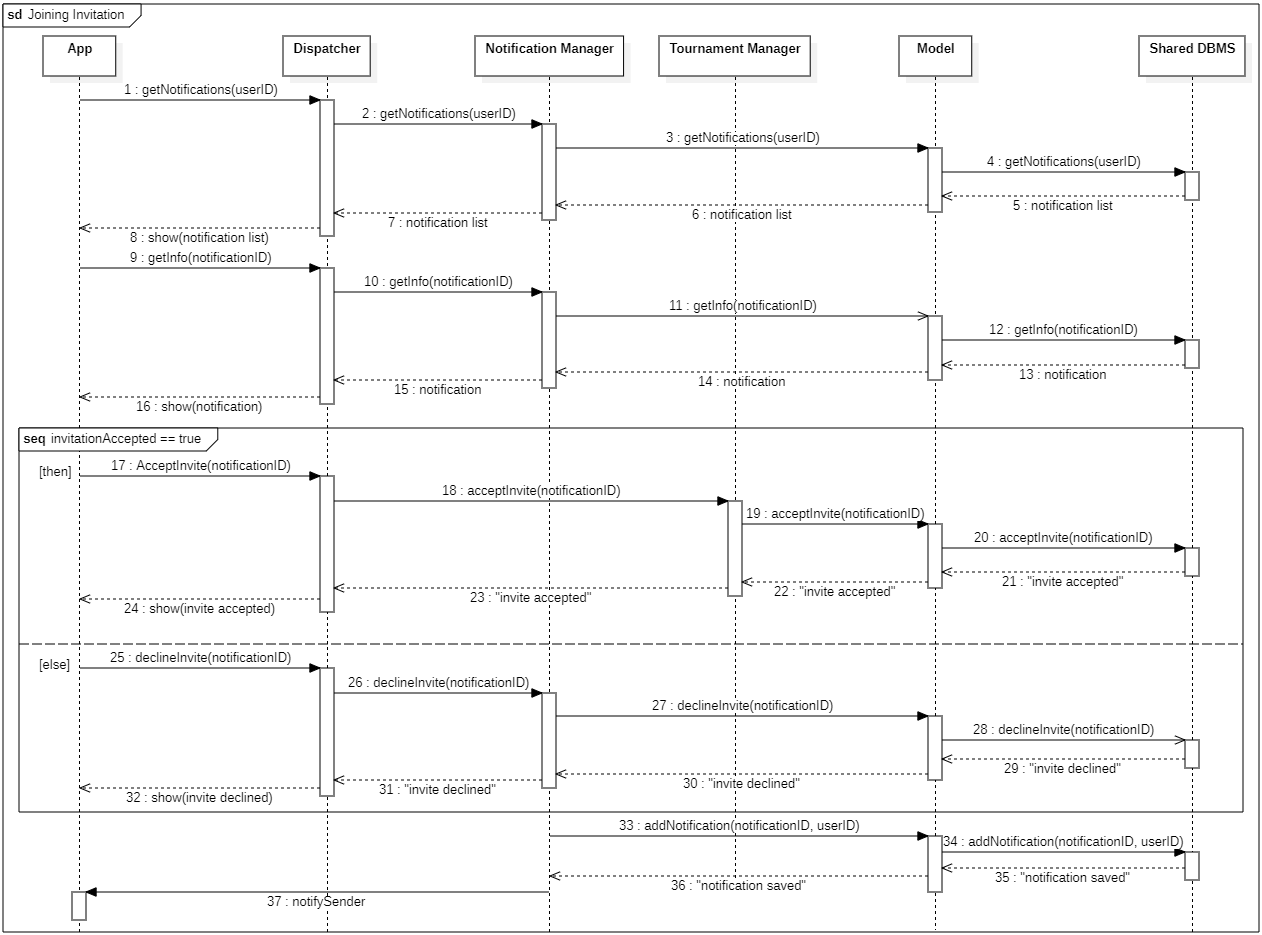
\includegraphics[width=\linewidth]{UC15.png}
\end{figure}
\noindent
This sequence diagram outlines the process of a user joining an invitation. Initially, the app sends a request to the Notification Manager to retrieve all active notifications from the Shared DBMS. Subsequently, the app requests information about a specific notification from the Notification Manager, which obtains the information by accessing the Shared DBMS. \\
If the user chooses to accept the invitation, the app sends a request to the Tournament Manager, which adds the user to the invited group. In the case of declining the invitation, the app sends a request to the Notification Manager, which handles the decline process. After the invitation is either accepted or declined, the Notification Manager creates a new notification, saves it in the Shared DBMS, and then sends the new notification to all designated users.

\begin{figure}[H]
    \centering
    \textbf{[UC16] Searching} \\
    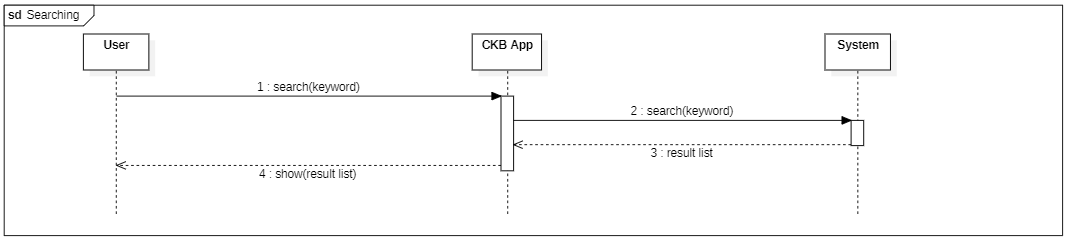
\includegraphics[width=\linewidth]{UC16.png}
\end{figure}
\noindent
This sequence diagram illustrates the user's search procedure involving the insertion of a specific keyword. The app sends a request to the Search Manager, which queries the Shared DBMS to retrieve a list of results for the specified keyword. The Search Manager then sends this list to the app.

\subsection{Component interfaces}

\subsection{Selected architectural styles and patterns}

\subsection{Other design decisions}


\section{User Interface Design}


\begin{figure}[H]
    \centering
    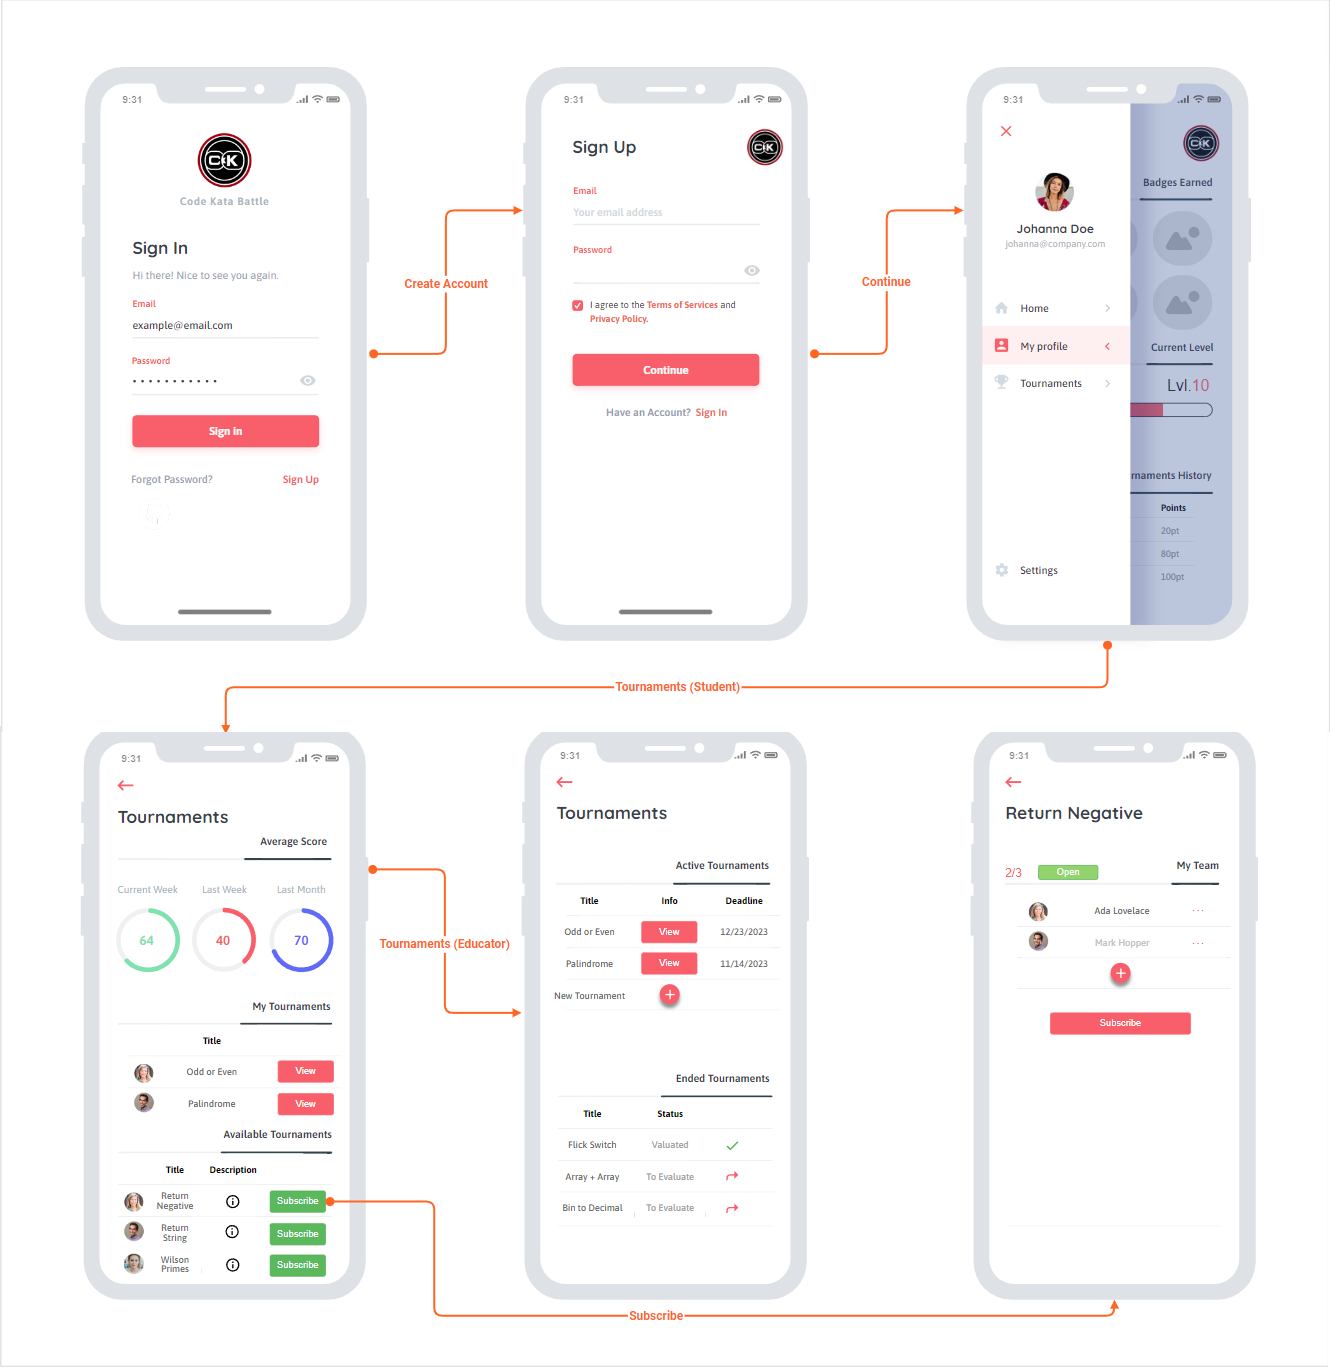
\includegraphics[width=\linewidth]{Mobile UI.png}
    \caption{General UI}
\end{figure}

\begin{figure}[H]
    \centering
    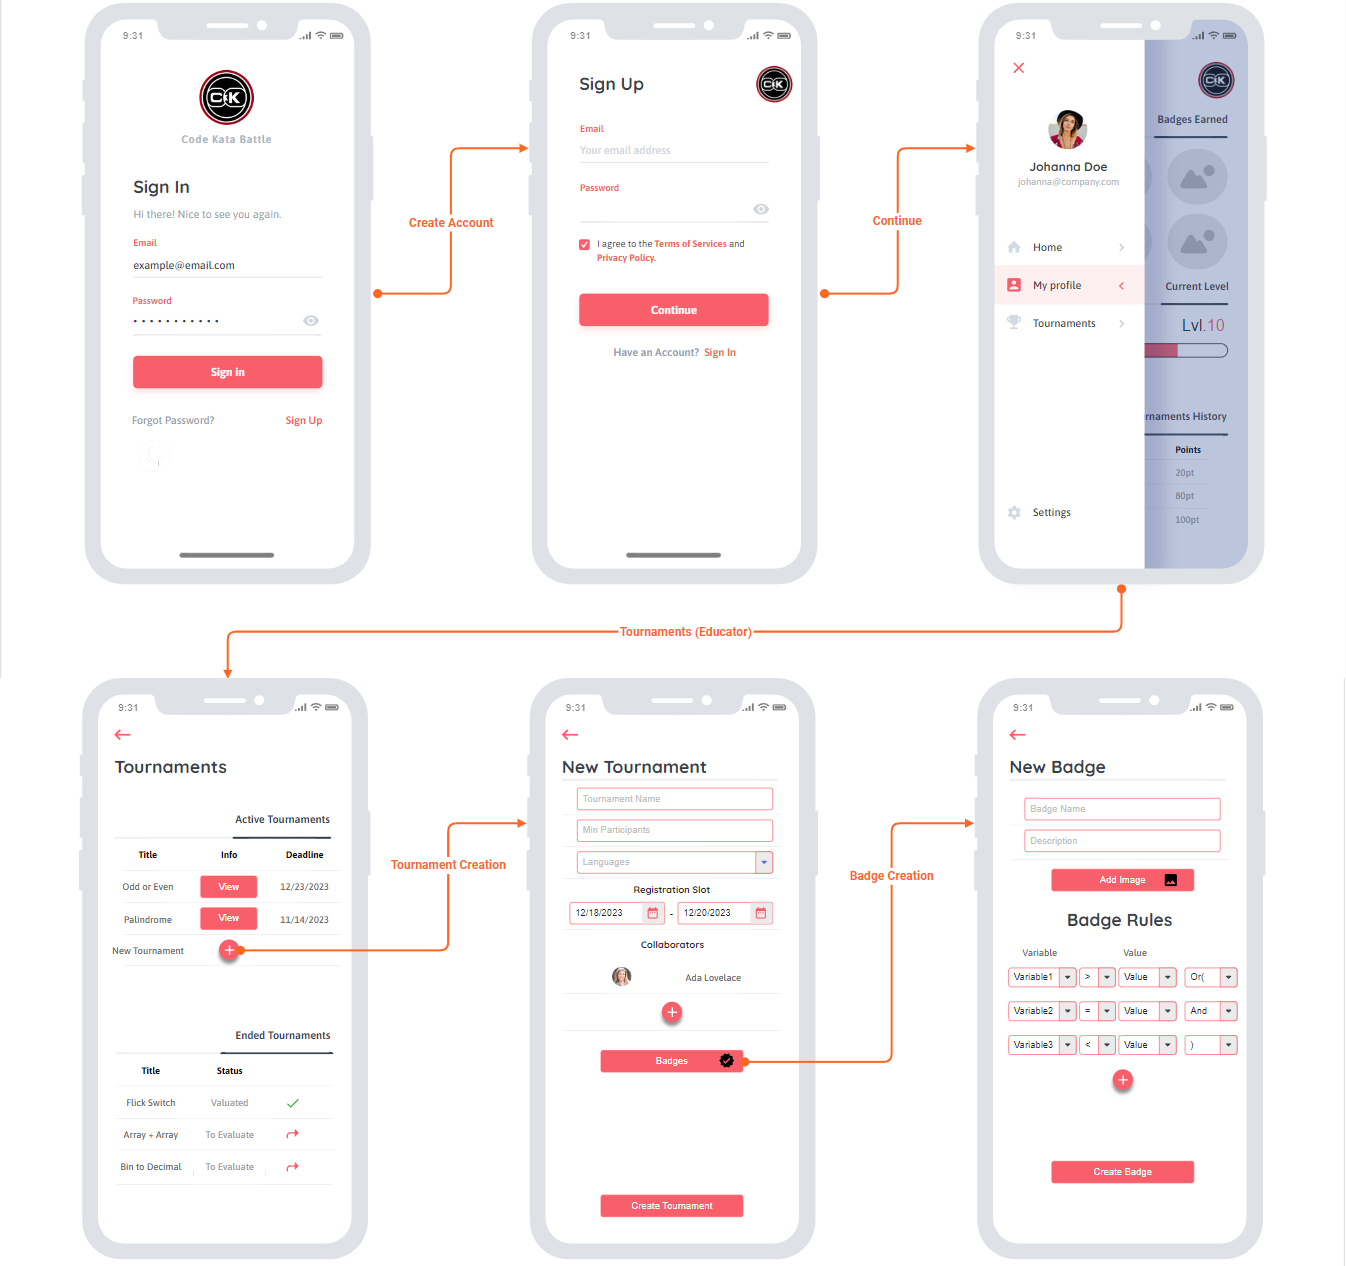
\includegraphics[width=\linewidth]{Mobile UI ED.png}
    \caption{Tournament and Badge creation}
\end{figure}

\begin{figure}[H]
    \centering
    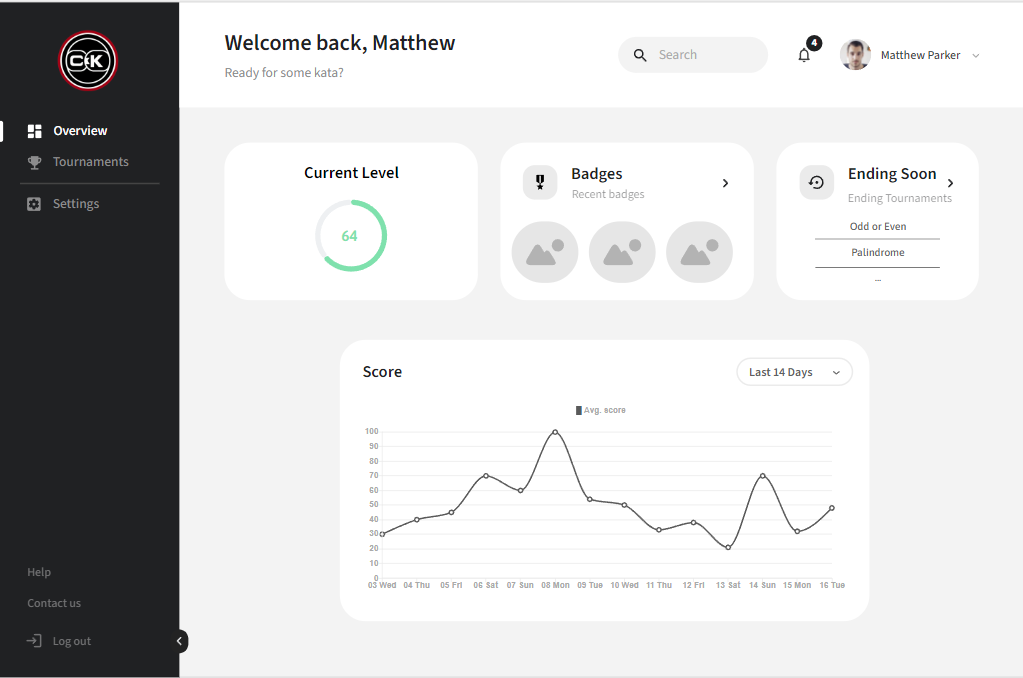
\includegraphics[width=\linewidth]{Web UI.png}
    \caption{Web UI Overview}
\end{figure}

\begin{figure}[H]
    \centering
    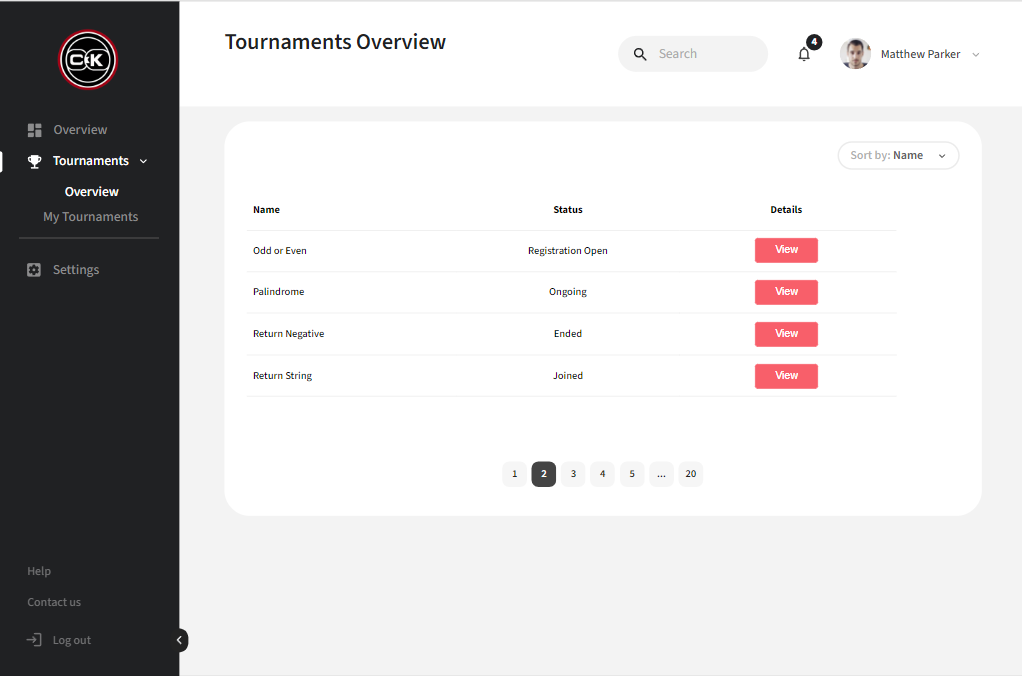
\includegraphics[width=\linewidth]{Web UI 2.png}
    \caption{Web UI Tournament Overview}
\end{figure}

\begin{figure}[H]
    \centering
    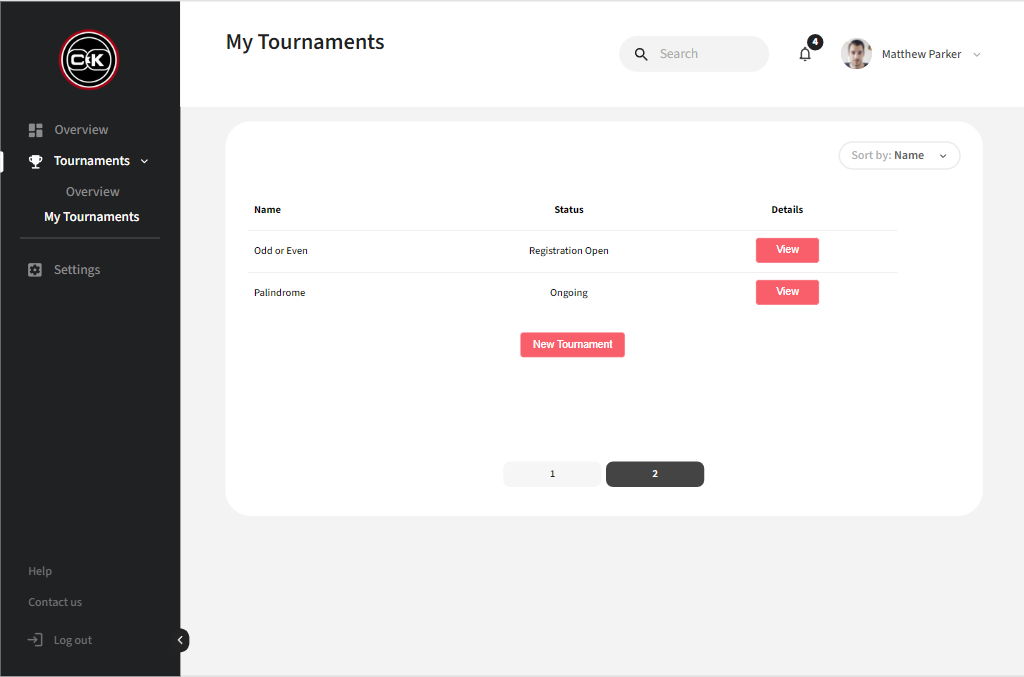
\includegraphics[width=\linewidth]{Web UI 3.png}
    \caption{Web UI My Tournament view}
\end{figure}

\begin{figure}[H]
    \centering
    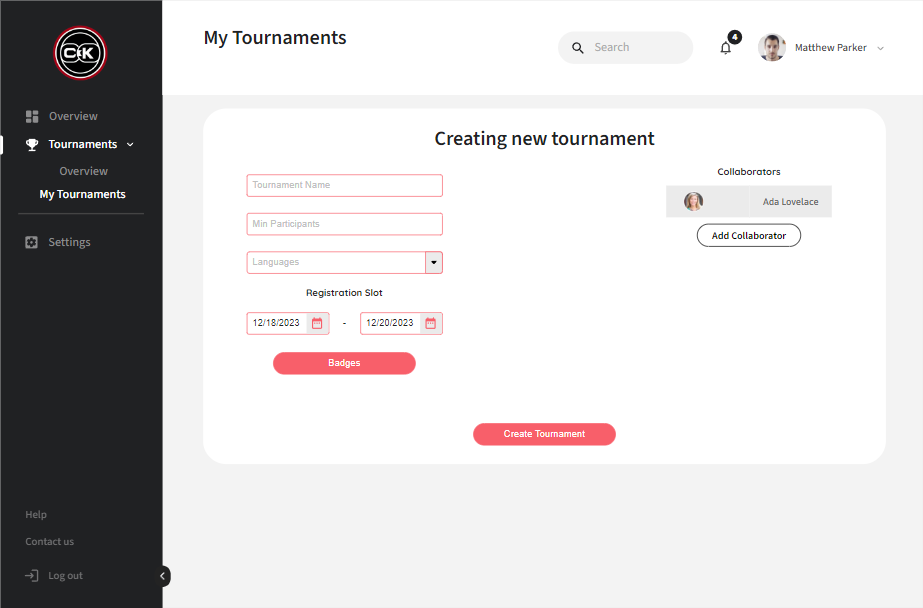
\includegraphics[width=\linewidth]{Web UI 4.png}
    \caption{Web UI Tournament creation view}
\end{figure}

\begin{figure}[H]
    \centering
    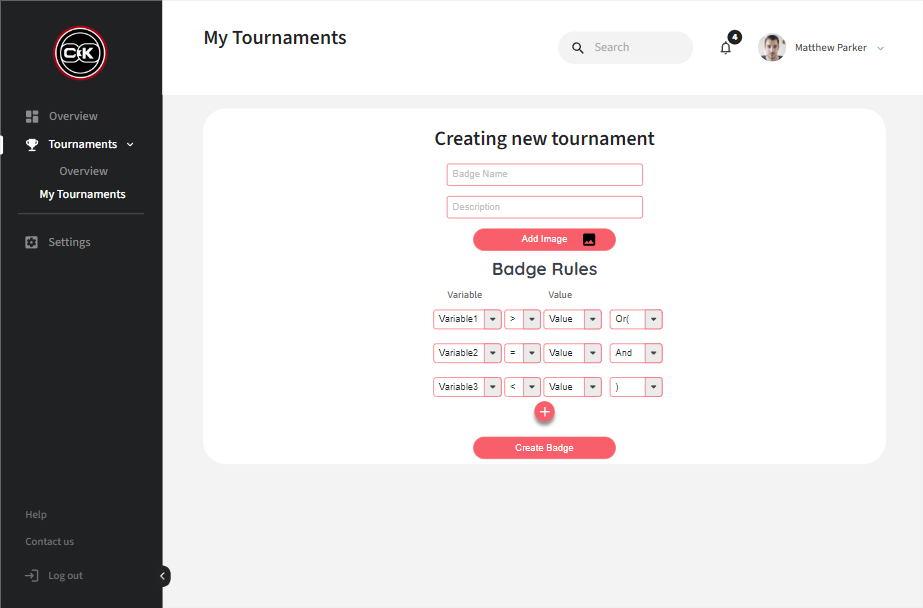
\includegraphics[width=\linewidth]{Web UI 5.png}
    \caption{Web UI Badge creation view}
\end{figure}

\section{Requirements Traceability}

\section{Implementation, Integration and Test Plan}

\section{Effort Spent}
\begin{center}
\textbf{Armando Fiorini} \\
\vspace{10px}
    \begin{tabularx}{0.8\textwidth} { 
  | >{\centering\arraybackslash}X 
  | >{\centering\arraybackslash}X | }
 \hline
 \textbf{Chapter} & \textbf{Hours Spent} \\
 \hline
 1 & TBD  \\
 \hline
 2 & TBD \\
 \hline
 3 & TBD \\
 \hline
 4 & TBD \\
 \hline
 5 & TBD \\
 \hline
\end{tabularx}

\vspace{10px}
\textbf{Samuele Motta} \\
\vspace{10px}
\begin{tabularx}{0.8\textwidth} { 
  | >{\centering\arraybackslash}X 
  | >{\centering\arraybackslash}X | }
 \hline
 \textbf{Chapter} & \textbf{Hours Spent} \\
 \hline
 1 & TBD  \\
 \hline
 2 & TBD \\
 \hline
 3 & TBD \\
 \hline
 4 & TBD \\
 \hline
 5 & TBD \\
 \hline
\end{tabularx}

\vspace{10px}
\textbf{Vajihe Gholami} \\
\vspace{10px}
\begin{tabularx}{0.8\textwidth} { 
  | >{\centering\arraybackslash}X 
  | >{\centering\arraybackslash}X | }
 \hline
 \textbf{Chapter} & \textbf{Hours Spent} \\
 \hline
 1 & TBD  \\
 \hline
 2 & TBD \\
 \hline
 3 & TBD \\
 \hline
 4 & TBD \\
 \hline
 5 & TBD \\
 \hline
\end{tabularx}

\end{center}

\section{References}

\end{document}
